\documentclass[]{article}
\usepackage{lmodern}
\usepackage{amssymb,amsmath}
\usepackage{ifxetex,ifluatex}
\usepackage{fixltx2e} % provides \textsubscript
\ifnum 0\ifxetex 1\fi\ifluatex 1\fi=0 % if pdftex
  \usepackage[T1]{fontenc}
  \usepackage[utf8]{inputenc}
\else % if luatex or xelatex
  \ifxetex
    \usepackage{mathspec}
  \else
    \usepackage{fontspec}
  \fi
  \defaultfontfeatures{Ligatures=TeX,Scale=MatchLowercase}
\fi
% use upquote if available, for straight quotes in verbatim environments
\IfFileExists{upquote.sty}{\usepackage{upquote}}{}
% use microtype if available
\IfFileExists{microtype.sty}{%
\usepackage{microtype}
\UseMicrotypeSet[protrusion]{basicmath} % disable protrusion for tt fonts
}{}
\usepackage[margin=1in]{geometry}
\usepackage{hyperref}
\PassOptionsToPackage{usenames,dvipsnames}{color} % color is loaded by hyperref
\hypersetup{unicode=true,
            pdftitle={Portfolio intuition},
            colorlinks=true,
            linkcolor=Maroon,
            citecolor=Blue,
            urlcolor=blue,
            breaklinks=true}
\urlstyle{same}  % don't use monospace font for urls
\usepackage{graphicx,grffile}
\makeatletter
\def\maxwidth{\ifdim\Gin@nat@width>\linewidth\linewidth\else\Gin@nat@width\fi}
\def\maxheight{\ifdim\Gin@nat@height>\textheight\textheight\else\Gin@nat@height\fi}
\makeatother
% Scale images if necessary, so that they will not overflow the page
% margins by default, and it is still possible to overwrite the defaults
% using explicit options in \includegraphics[width, height, ...]{}
\setkeys{Gin}{width=\maxwidth,height=\maxheight,keepaspectratio}
\IfFileExists{parskip.sty}{%
\usepackage{parskip}
}{% else
\setlength{\parindent}{0pt}
\setlength{\parskip}{6pt plus 2pt minus 1pt}
}
\setlength{\emergencystretch}{3em}  % prevent overfull lines
\providecommand{\tightlist}{%
  \setlength{\itemsep}{0pt}\setlength{\parskip}{0pt}}
\setcounter{secnumdepth}{0}
% Redefines (sub)paragraphs to behave more like sections
\ifx\paragraph\undefined\else
\let\oldparagraph\paragraph
\renewcommand{\paragraph}[1]{\oldparagraph{#1}\mbox{}}
\fi
\ifx\subparagraph\undefined\else
\let\oldsubparagraph\subparagraph
\renewcommand{\subparagraph}[1]{\oldsubparagraph{#1}\mbox{}}
\fi

%%% Use protect on footnotes to avoid problems with footnotes in titles
\let\rmarkdownfootnote\footnote%
\def\footnote{\protect\rmarkdownfootnote}

%%% Change title format to be more compact
\usepackage{titling}

% Create subtitle command for use in maketitle
\newcommand{\subtitle}[1]{
  \posttitle{
    \begin{center}\large#1\end{center}
    }
}

\setlength{\droptitle}{-2em}
  \title{Portfolio intuition}
  \pretitle{\vspace{\droptitle}\centering\huge}
  \posttitle{\par}
  \author{Chris Kennedy\\
Bridge Alternatives\\
\href{mailto:chris.kennedy@bridgealternatives.com}{\nolinkurl{chris.kennedy@bridgealternatives.com}}}
  \preauthor{\centering\large\emph}
  \postauthor{\par}
  \predate{\centering\large\emph}
  \postdate{\par}
  \date{June 21, 2018}

\usepackage{fancyhdr}
\pagestyle{fancy}

\makeatletter
\lhead{\@title}
\rhead{
\includegraphics[width = 0.15\textwidth]{logo.png}}
\makeatother

\begin{document}
\maketitle

\hypertarget{introduction}{%
\subsection{Introduction}\label{introduction}}

There's a short preference test in this paper that most readers, if not
all, will answer incorrectly. It's a ``preference test'' (and not a
quiz) because selections should be made without calculation or
computation. I'm looking to test your intuition.

Below I argue for why we should care about where our intuition is
leading us, why it might be creating blind spots and how we can do
better. Specifically, I attempt to demonstrate the limitations of
financial judgement based on return to risk ratios (i.e.~Sharpe ratios)
and how something like this might be better:

\[
\frac{RRR_a}{\rho} > RRR_p
\]

\[
RRR_a > \rho \times RRR_p
\]

Don't worry, we'll come back to these.

\hypertarget{intuition}{%
\subsection{Intuition}\label{intuition}}

Practitioners in the hedge fund industry must often rely on intuition.
In some ways, given the highly quantitative nature of the industry, this
is surprising; in other ways it isn't. The types of problems regularly
encountered can be extremely complicated, requiring involved computation
for, at best, reasonable approximations. Successful individuals develop
heuristics (shortcuts) to more efficiently guide their day-to-day
filtering of opportunities. They develop a sense for what should foot
and what shouldn't. It's an element of discretion, molded by experience,
that manifests in small but important decisions across the sector
everyday:

\begin{itemize}
\tightlist
\item
  Does this manager's presentation warrant follow up?
\item
  Does this line of research show promise?
\item
  How do I feel about the risk we're taking?
\item
  Does this make sense?
\end{itemize}

Granted, these are questions we'd ideally approach quantitatively, but
this takes time we don't always have.

A common instance of this discretion is visible in the evaluation of
performance statistics. Hedge fund investors are confronted with an
amazing amount of data: daily returns, monthly returns, return
statistics, sector exposures, positions, correlation matrices and more.
Given this mountain of information, it's necessary to employ time saving
tools to filter true prospects from everything else.

One such tool is the return to risk ratio (\(RRR\)). It might seem
strange to call the \(RRR\) a ``tool,'' especially in the context of
shortcuts and heuristics, since the ratio has such a strong theoretical
source: William Sharpe\footnote{Yes, this is a slight inaccuracy.
  Sharpe's namesake ratio incorporated the risk free rate, but the idea
  of dimensionalizing returns using risk is what's important here.}. But
it helps to remember that the \(RRR\) is, indeed, a deliberate
simplification, facilitating the comparison of assets of different risks
``as long as the correlations of the {[}assets{]} with other relevant
asset classes are reasonably similar''
(\href{https://web.stanford.edu/~wfsharpe/art/sr/sr.htm}{Sharpe's
words}). So while the \(RRR\) and Sharpe ratio have their limitations,
you'd be hard pressed to find any presentation of hedge fund performance
that didn't show them. The statistic carries an importance, a currency,
derived from its simplicity and implication of skill---even though
confidently quantifying ``skill'' is probably more complicated.

In the next section, you'll be asked to put yourself in the shoes of a
portfolio manager. You'll be presented with a series of investment
preference tests designed to examine your ability to pick superior
assets. It will be tempting to reach for a spreadsheet or Python or R,
but don't. Try and let intuition guide you. And while this may feel
frivolous, if you were ever presented with statistics describing some
potential investment and, without deliberately calculating its potential
impact on your portfolio, decided it wasn't for you, then you've made
choices like this before.

\hypertarget{preference-tests}{%
\subsection{Preference Tests}\label{preference-tests}}

Below are four preference tests where you'll need to pick one of two
assets (i.e. \(A_1\) or \(A_2\); \(B_1\) or \(B_2\); etc.). In each,
assume you already own a portfolio that exhibits a return of 5\% and a
risk of 15\%. Also, pretend you're seeking to allocate capital such that
the resulting weights will be split 90\% to your current portfolio and
10\% to your asset choice. This asset will therefore play a small but
not unimportant role in the new portfolio. Lastly, assume you're
objective is to maximize your portfolio's return over risk ratio
(\(RRR\)).\footnote{It's perfectly reasonable to prefer some other
  objective function. The \(RRR\), while mathematically flexible, has
  some practical limitations. For instance, the maximized \(RRR\) might
  exhibit a very low return. But the spirit of this work---attempting to
  distill portfolio goals into simple but complete tools and guides---is
  extendable to any objective function.}

\[
\begin{array}{r|c|c|c}
\text{}                   & A_1    & or & A_2 \\
\hline{}
\text{Return }(r)       & 4.00\% &    & 4.00\% \\
\text{Risk }(\sigma)      & 7.96\% &    & 46.04\% \\
\text{Correlation }(\rho) & -0.2   &    & -0.2
\end{array}
\]

\[
\begin{array}{r|c|c|c}
\text{}                   & B_1     & or & B_2  \\
\hline
\text{Return }(r)       & 10.54\% &    & 3.57\% \\
\text{Risk }(\sigma)      & 20.00\% &    & 20.00\% \\
\text{Correlation }(\rho) & 0.8     &    & -0.2
\end{array}
\]

\[
\begin{array}{r|c|c|c}
\text{}                   & C_1     & or & C_2 \\
\hline{}
\text{Return }(r)       & 9.33\%  &    & 6.50\% \\
\text{Risk }(\sigma)      & 27.50\% &    & 12.50\% \\
\text{Correlation }(\rho) & 0.4     &    & 0.4
\end{array}
\]

\[
\begin{array}{r|c|c|c}
\text{}                   & D_1     & or & D_2 \\
\hline{}
\text{Return }(r)       & 6.43\%  &    & -2.64\% \\
\text{Risk }(\sigma)      & 10.00\% &    & 40.00\% \\
\text{Correlation }(\rho) & 0.5     &    & -0.6
\end{array}
\]

After presenting this test to several people, a typical set of answers
started to emerge:

\begin{enumerate}
\def\labelenumi{\arabic{enumi}.}
\tightlist
\item
  \(A_1\) was preferred to \(A_2\). With \(A_1\), for the same return
  and correlation, you receive nearly 6 times less risk.
\item
  \(B_1\) was slightly preferred to \(B_2\). For the same risk, \(B_1\)
  delivers much more return, though \(B_2\)'s correlation is better.
\item
  \(C_2\) was preferred. It's \(RRR\) is higher (about 0.52 versus about
  0.34).
\item
  \(D_1\) was preferred to \(D_2\). \(D_1\)'s return to risk ratio
  (\(RRR\)) is much higher. \(D_2\)'s return is negative.
\end{enumerate}

\hypertarget{results}{%
\subsection{Results}\label{results}}

To reveal the results and see how far intuition can get you, we'll start
with the case of \(A_1\) and \(A_2\), which should exhibit the most
consensus. Most, if not all, will have chosen \(A_1\) over \(A_2\). For
the same return and correlation you receive much, much less risk. Let's
calculate the portfolio impact of each investment and see exactly how
much better you are with \(A_1\) over \(A_2\):

\hypertarget{portfolio-return-r}{%
\subsubsection{Portfolio Return (R)}\label{portfolio-return-r}}

Since the returns of the prospective assets \(A_1\) and \(A_2\) are
identical, the resulting portfolio returns will be identical as well:

\[
\begin{aligned}
R & = w_p r_p + w_a r_a \\
R & = 0.9 \times 0.05 + 0.1 \times 0.04 \\
R & = 0.049 \\
\end{aligned}
\]

\[
\begin{aligned}
Where: & \\
R & = \text{return of the portfolio after allocating to the prospective asset} \\
r_p & = \text{return of the current portfolio} \\
r_a & = \text{return of the prospective asset} \\
w_p & = \text{weight of the current portfolio post-allocation} \\
w_a & = \text{weight of the prospective asset post-allocation} \\
w_a & = (1 - w_p)
\end{aligned}
\]

\hypertarget{portfolio-risk-s}{%
\subsubsection{Portfolio Risk (S)}\label{portfolio-risk-s}}

Now, because the risks of \(A_1\) and \(A_2\) are so different, we
expect a logical preference to very clearly emerge below. We'll first
calculate the portfolio's resulting risk (\(S\)) for \(A_1\):

\[
\begin{aligned}
S & = \sqrt{w_p^2 \sigma_p^2 + w_a^2 \sigma_a^2 + 2 w_p w_a \sigma_p \sigma_a \rho} \\
S & = \sqrt{(0.9 \times 0.15)^2 + (0.1 \times 0.0796)^2 + 2 \times 0.9 \times 0.1 \times 0.15 \times 0.0796 \times -0.2} \\
S & = \sqrt{0.018225 + 0.0000633616 - 0.00042984} \\
S & = \sqrt{0.0178585216} \\
S & = 0.13363577964 \\
S & \approx 13.363...\% 
\end{aligned}
\]

\[
\begin{aligned}
Where: & \\
S & = \text{risk of the portfolio after allocating to the prospective asset} \\
\sigma_p & = \text{risk of the current portfolio} \\
\sigma_a & = \text{risk of the prospective asset} \\
\rho & = \text{correlation between the current portfolio and the prospective asset} \\
\end{aligned}
\]

If we take the ratio of \(R\) to \(S\), the resulting portfolio's
\(RRR\) is now about 0.3667, which represents a 10\% improvement. Not
bad.

Let's see how much better that is than \(A_2\):

\[
\begin{aligned}
S & = \sqrt{w_p^2 \sigma_p^2 + w_a^2 \sigma_a^2 + 2 w_p w_a \sigma_p \sigma_a \rho} \\
S & = \sqrt{(0.9 \times 0.15)^2 + (0.1 \times 0.4604)^2 + 2 \times 0.9 \times 0.1 \times 0.15 \times 0.4604 \times -0.2} \\
S & = \sqrt{0.018225 + 0.0021196816 - 0.00248616} \\
S & = \sqrt{0.0178585216} \\
S & = 0.13363577964 \\
S & \approx 13.363...\% 
\end{aligned}
\]

\hypertarget{um-what}{%
\subsection{Um, what?}\label{um-what}}

There are no tricks here. Feel free to replicate the math yourself.
You'll find that \(A_1\) and \(A_2\) deliver the exact same change to
the portfolio's risk, which, since their returns are identical, results
in the same +10\% change to the portfolio's \(RRR\).\footnote{It should
  be noted that, in an ideal scenario, we'd have transparency into the
  constituency of the current portfolio, and that's obviously not
  provided here. The portfolio's particular makeup could influence
  allocation decisions, likely affecting choices about weightings or
  even the binary question of inclusion. In the scenario painted in this
  paper, we implicitly assume the portfolio manager cannot see their own
  portfolio's inner-workings. This clear limitation may be a relatable
  one, though. How often does a portfolio manager within a large
  institution (like a pension fund) have access to, or the ability to
  affect, other parts of the portfolio? So while this is indeed a
  shortcut, it's a fair one that allows us to make progress. I'd add two
  more points: (1) prioritizing opportunities based on Sharpe ratios
  ignores the portfolio's inner workings too, and (2) this paper is not
  proposing a better way to optimize portfolio weights but only a fairer
  way to quickly filter opportunities.}

Think about that. We essentially took an asset (\(A_1\)), added nearly
40\% more risk and ended up with the same resulting portfolio. How's
that possible? Look at the formula for the post-allocation risk (\(S\)),
specifically the last two terms: \(w_a^2 \sigma_a^2\) and
\(2 w_p w_a \sigma_p \sigma_a \rho\). Respectively, these items describe
risk contributions from the prospective asset individually and in
combination with the original portfolio. As we increase the asset's
risk, the first term grows exponentially, and the second term shrinks
linearly (remember, the correlation is negative). It turns out that, at
least temporarily, the shrinking effect from the negative correlation
outweighs the exponential term. We can show this graphically by plotting
how these terms and their sum change as we adjust the asset's risk:

\begin{center}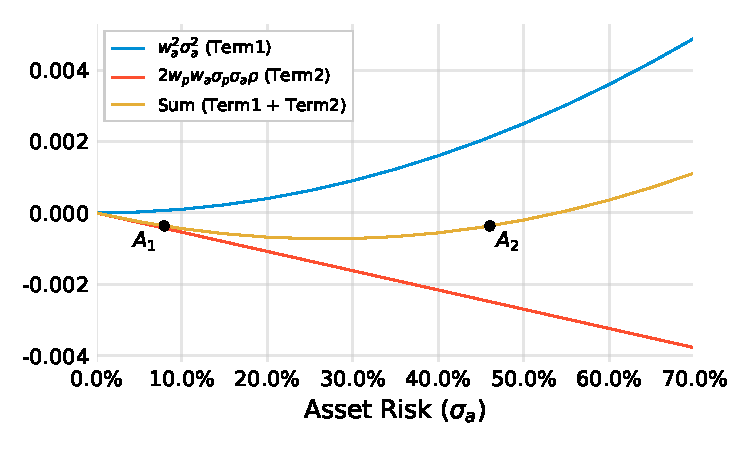
\includegraphics{paper_files/figure-latex/Risk terms-1} \end{center}

For a while, the red line, which describes the risk reduction from the
negatively correlated combination, wins out, allowing for pairs like
\(A_1\) and \(A_2\).

When I first discovered the math behind these strange asset pairs (see
the Appendix for more details), I remember feeling uneasy. We're
strongly trained to view more risk, holding all else constant, as a bad
thing. In some ways, it's a sort of tenant of sound financial thinking.
But here, in this example, that's just not the case.

I doubt at this point you'll be too surprised to learn that all the
other assets in the preference test also deliver the exact same 10\%
improvement to the portfolio's return to risk ratio. Each asset from the
test is, from a quantitative perspective, equivalent. You were right
(and wrong) whatever you picked.

\hypertarget{visualizing-equivalence}{%
\subsection{Visualizing equivalence}\label{visualizing-equivalence}}

In order to make sense of the equivalence behind these seemingly
disparate assets, let's first plot each them in a risk-return space:

\begin{center}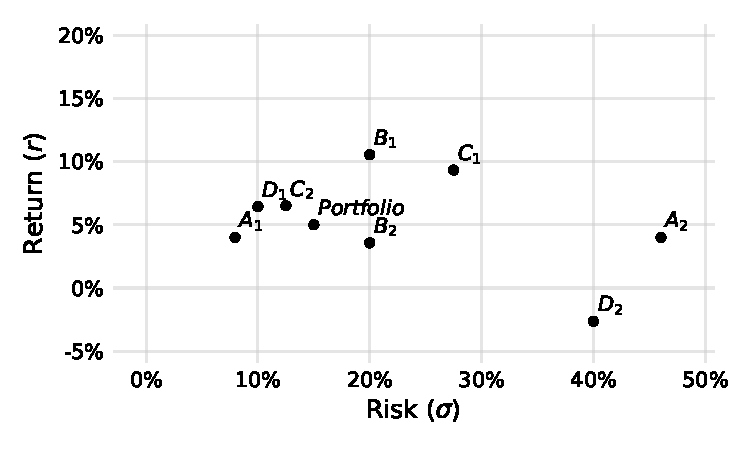
\includegraphics{paper_files/figure-latex/Scatter-1} \end{center}

At first glance it's hard to see the ``equivalence.'' Looking at this
plot, it is natural to gravitate towards points higher and to the left.
In this light, \(A_1\), \(D_1\), \(C_2\), \(B_1\) look preferential. And
if the \(RRR\) of each asset is our sole consideration, then these truly
are preferential assets. But the story is incomplete without considering
correlation. When we do that, the picture begins to take shape:

\begin{center}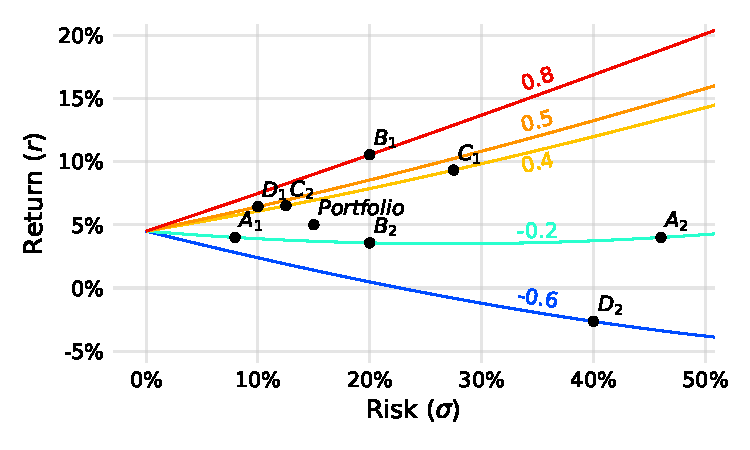
\includegraphics{paper_files/figure-latex/Scatter with correlation lines-1} \end{center}

Each line drawn in this plot represents a class of assets that:

\begin{enumerate}
\def\labelenumi{\arabic{enumi}.}
\tightlist
\item
  Share some correlation to the portfolio (0.8, 0.5, 0.4, -0.2, or -0.6)
\item
  Deliver a 10\% improvement, measured in \(RRR\), to the original
  portfolio when allocated at a 10\% weight
\end{enumerate}

With the added correlation lines it's easier to see how, as the
correlation drops (corresponding to lines of ``cooler'' coloring), less
return is required to deliver the same 10\% improvement. Put
differently, return is traded for lower correlation such that the
resulting portfolio improvement remains constant.

Correlation is what connects these assets. While that's obvious now, it
wasn't when you were selecting preferences. Whatever you picked, you
still picked, and I think this proves two important things:

\begin{enumerate}
\def\labelenumi{\arabic{enumi}.}
\tightlist
\item
  How difficult it is to internalize correlation
\item
  At the same time, how important correlation really is
\end{enumerate}

This is a problem, right? \(RRR\)'s and Sharpe ratios are mentally
portable. They are easy, compact and can be helpful when correlations
are ``reasonably similar.'' But even by that logic you'd have developed
illogical preferences for \(A_1\) (over \(A_2\)) and \(C_2\) (over
\(C_1\)). It seems, especially within the world of hedge funds where
lower correlations to traditional assets are more common, something
better is required that:

\begin{enumerate}
\def\labelenumi{\arabic{enumi}.}
\tightlist
\item
  Incorporates correlation
\item
  Remains simple to calculate
\end{enumerate}

Luckily, I develop just the formula below. While being remarkably
simple, the formula is surprisingly difficult to derive, which may
explain why I haven't seen it used much. Starting with the idea of an
indifference curve, I'll reveal the intuition and a bit of the math
behind the derivation.

\hypertarget{indifference-curves}{%
\subsection{Indifference curves}\label{indifference-curves}}

An indifference curve, in the traditional context of economics, connects
combinations of variables into a curve for which a consumer is
indifferent. They are indifferent because each point on one of these
curves corresponds to the same level of utility or happiness or reward.

In the context of portfolio mathematics we'll connect combinations of
prospective asset return, risk and correlation for which an allocator is
indifferent. Since the idea of utility translates nicely into \(RRR\)s
(we're generally happier with more return per unit of risk), what we're
really examining are different kinds of prospective assets that deliver
the exact same change to the portfolio. And this should sound familiar.
In the preference test, we constructed a set of 8 assets that exhibited
very different returns, risks and correlations, for which we were
indifferent; they all delivered the same +10\% change to the portfolio's
\(RRR\).

To derive the new formula, we'll focus not on assets that deliver a
+10\% change, but those that deliver no change. This is a little
confusing since it's hard to see the practical value of such an
exercise. Essentially these are assets that, when added at some weight
(\(w_a\)), do not change the portfolio's return over risk. It's
important to realize that such an asset doesn't have to be identical to
the portfolio with a correlation of 1.0. It can exhibit any correlation
or risk or return subject to some quantitative constraints. For instance
if some prospective asset delivers relatively low return, it will
obviously lower the portfolio's return. It must balance this with
attractive (i.e.~low) correlation that will serve to reduce the
portfolio's risk. If the risk is lowered enough as to offset the lower
return, the ratio of the two is preserved and the portfolio's \(RRR\) is
unchanged.

We can express this idea formally:

\[
\frac{r_p}{\sigma_p} = \frac{w_p r_p + w_a r_a}
{\sqrt{w_p^2 \sigma_p^2 + w_a^2 \sigma_a^2 + 2 w_p w_a \sigma_p \sigma_a \rho}}
\]

\[
\begin{aligned}
Where: & \\
r_p & = \text{return of the current portfolio} \\
r_a & = \text{return of the prospective asset} \\
\sigma_p & = \text{risk of the current portfolio} \\
\sigma_a & = \text{risk of the prospective asset} \\
\rho & = \text{correlation between the current portfolio and the prospective asset} \\
w_p & = \text{weight of the current portfolio post-allocation} \\
w_a & = \text{weight of the prospective asset post-allocation} \\
w_a & = (1 - w_p)
\end{aligned}
\]

The left hand side of the equation is just the current, pre-allocation
portfolio's return over risk. It's the starting point. We're interested
in the class of prospective assets that, when combined with the
portfolio at a particular weight (\(w_a\)), do not change the original
return over risk. We can call these ``do no harm'' or ``no change''
assets. Since this class of assets all essentially do nothing, we're not
only indifferent to which member of the class we choose, but whether we
choose one or not. Whatever we do, it doesn't make a difference; the
portfolio's return over risk will remain the same.

\hypertarget{so-why-are-we-interested-at-all}{%
\subsection{So why are we interested at
all?}\label{so-why-are-we-interested-at-all}}

Good question. Let's first graph these curves and get back to that.

\begin{center}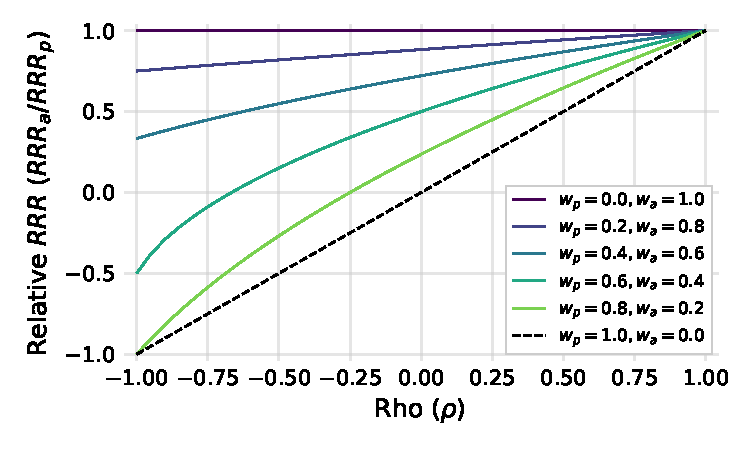
\includegraphics{paper_files/figure-latex/Indifference curves-1} \end{center}

Each of these lines is an indifference curve, representing different
kinds of those ``no change'' assets, drawn for a particular portfolio
weight (\(w_p\)). Every portfolio weight implies an allocation weight
(\(w_a\)) since \(w_a = 1 - w_p\). The x-axis here is simply the
correlation between the portfolio and prospective asset. The y-axis
captures the relative return to risk of the asset when compared to the
portfolio. When the \(Relative\ RRR\) is:

\begin{itemize}
\tightlist
\item
  = 1, the the return over risk ratios of the asset and portfolio are
  the same
\item
  \textgreater{} 1, the return over risk ratio of the asset is greater
  than the portfolio
\item
  \textless{} 1, the return over risk ratio of the asset is less than
  the portfolio
\end{itemize}

Notice how, as the weight allocated to the asset increases (the lines
move upward, from green to purple), the asset must be more performant in
order to do no harm; it must be better relative to the portfolio. Put
differently, as the role played by the asset increases, more is required
of it, and that sounds about right.

If we go the other way and shrink the weight allocated to the
prospective asset, we obviously reduce what's required of it. It turns
out, as a consequence of the math, that if we allow the weight allocated
to approach but not equal zero (illustrated by the dashed line), we're
left with an amazingly concise limiting scenario:

\[
\frac{RRR_a}{RRR_p} = \rho
\]

\[
\begin{aligned}
Where: & \\
RRR_p & = \text{return to risk ratio of the current portfolio}\ (r_p / \sigma_p) \\
RRR_a & = \text{return to risk ratio of the prospective asset}\ (r_a / \sigma_a) \\
\rho & = \text{correlation between the current portfolio and the prospective asset} \\
\end{aligned}
\]

This formula describes what's required, in an absolute bare-minimum
mathematical sense, of a prospective asset in order to do no harm. If
for some reason the asset's correlation goes up or its \(RRR\) down, by
any amount, we know that the asset will only harm the portfolio
irrespective of the weight chosen.

Take a minute to appreciate the brevity. Just three terms are required
to answer this question: ``What is required from an asset (in terms of
return, risk and correlation) in order to add value to my portfolio?'' I
think that's awesome.

Since we'd like to be better than the bare-minimum, we can add an
inequality to this expression and rearrange it in two ways in order to
reinforce its pracital usability:

\[
\frac{RRR_a}{\rho} > RRR_p
\]

\[
RRR_a > \rho \times RRR_p
\]

Given your own portfolio's return over risk, the return over risk of
some prospective asset and how they correlate, you can immediately
determine if the asset will be able to add value. That's powerful and
simple.

For example, assume you still hold the 5\% return and 15\% risk
portfolio from the preference test. Let's say you've just been presented
with an investment opportunity that exhibits a 0.7 correlation to your
portfolio and a return to risk ratio of 0.2, which isn't great but
probably sounds additive. Using the first arrangement, we know that the
quotient of \(RRR_a\) and \(\rho\) must be greater than \(RRR_p\). When
we divide 0.2 by 0.7, we're left with about 0.286, which is actually
less than 0.333. Using the second arrangement, we know that the product
of \(RRR_p\) and \(\rho\) must be less than \(RRR_a\). When we multiply
0.7 and 0.333, we're predictably left with about 0.231, which is not
less than 0.2. Therefore, at any weight, we know this asset will reduce
the return to risk ratio of the portfolio and probably shouldn't be
where we focus our effort.

\hypertarget{interpretations}{%
\subsection{Interpretations}\label{interpretations}}

It's worth noting a few points about this inequality. First, as far as I
can tell, it cannot be used to somehow rank prospective assets. It can
only serve as a binary filter: yes or no. This might feel like a real
limitation. \(RRR\)s are absolutely rankable. They are measurements of
the same unit (risk). But as we've shown in this paper, those rankings
are not indicative of their true value within the context of a
portfolio. Making decisions based only on return and risk is like
ranking runners based on their times without asking how far they ran. It
doesn't make sense. If you take away one thing from this paper, this
should be it!

Second, correlation is best understood as a sort of performance hurdle.
For assets exhibiting low correlation, less is required of their
standalone performance (i.e.~return over risk), all else equal. In fact,
plug zero correlation into the second inequality and you get: \(RRR_a\)
\textgreater{} 0. This means that if you happen to find a truly
zero-correlation asset it will be additive as long as it has positive
returns.\footnote{Correlation, at least compared to return and risk, is
  a relatively unstable measurement. Its measurement error is
  comparatively large. This is a result of the math that defines it.
  Interestingly, our portfolio is relatively stable with respect to
  changes in correlation. Since we never realize our exact expectation
  of return, risk and correlation (we get a draw from the distribution
  instead), both of these effects should be considered in practical
  applications. This is an area I hope to write more about soon.}

Lastly, return over risk can still be helpful. If you look back at the
chart, you'll see that we don't plot relative \(RRR\)s that are greater
than one. These points correspond to prospective asset \(RRR\)s that are
greater than our portfolio's. The point is that if you find an asset
whose \(RRR\) is greater than your portfolio's, it will add value
regardless of the correlation. But that's not justification for focusing
solely on return over risk. If you are managing a well diversified
portfolio you should, by definition, struggle to find these better
performing assets. You'll more likely need to add value using assets
that exhibit \(RRR\)s which are less than what you already have.

\hypertarget{implications}{%
\subsection{Implications}\label{implications}}

Even though we've been writing about them for years\footnote{Burghardt,
  Walls \emph{Managed futures for Institutional Investors (Chapter 12:
  Superstars versus Teamwork)}. If you'd like a copy of this work,
  please email me.}, we know return to risk ratios and Sharpe ratios are
not going anywhere. That's fine, but we do hope that people remain
cognizant of their limitations. Those specific limitations were made
very obvious in the above preference test.

I hope this work helps practitioners remain mindful of correlation when
evaluating potential portfolio changes. Using the formulas derived just
above, I believe that task becomes easier, but it does require the
standard conversation to change somewhat. In particular, I think hedge
fund investors/allocators should be more open with their portfolio
returns. These are often highly diversified portfolios. The risk of
reverse engineering individual allocations or positions is very low, and
the upside of prospective investments being prepared with their unique
correlations to your portfolio is real.

Likewise, hedge fund managers shouldn't be afraid to ask for an
investor's benchmarks and/or their performance. Bring correlation to the
conversation more often, for it's an important and maybe
underappreciated avenue for value delivery and differentiation.

\hypertarget{references}{%
\subsection{References}\label{references}}

\begin{enumerate}
\def\labelenumi{\arabic{enumi}.}
\tightlist
\item
  I'm very thankful for the many colleagues and friends who provided a
  patient, helpful ear during the writing of this. In particular, Steve
  Evans from Tudor and Adrian Etoveric from Episteme Capital Partners
  were very generous with their time and feedback.
\item
  Parts of this work (primarily the idea of Sharpe indifference curves)
  were influenced by a wonderful presentation from Roy Niederhoffer of
  \href{https://www.niederhoffer.com/}{R. G. Niederhoffer Capital
  Management}, given during the 2016 \href{https://timesummit.org/}{time
  Summit}.
\item
  In the process of writing this, I came across
  \href{https://pdfs.semanticscholar.org/c094/f7fd32f6e5c36f121a0d246d6127587a473a.pdf}{related
  and interesting work} from Marcos De Prado and David Bailey of the
  Lawrence Berkeley National Laboratory. They are motivated by similar
  observations and arrive at comparable conclusions.
\end{enumerate}

\hypertarget{appendix}{%
\subsection{Appendix}\label{appendix}}

\(A_1\) and \(A_2\) are examples of an interesting subset of solutions
to the two asset functions for return and risk. Yes, these are somewhat
fun and surprising demonstrations of portfolio math, but they also
reveal how it can be logical, in certain situations, to want more risk
from an investment, all else equal. That's fun too.

Let's start with a plot of \(A_1\) and \(A_2\):

\begin{center}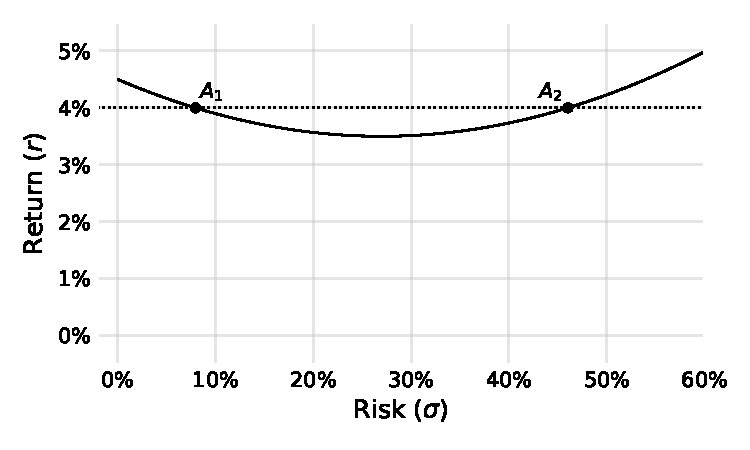
\includegraphics{paper_files/figure-latex/A1 A2-1} \end{center}

The line in this plot connects assets that, just like \(A_1\) and
\(A_2\), deliver a +10\% change with a correlation of -0.2. And since
this line is a parabola, we can, in certain situations, find two asset
risks (i.e.~solutions) given a particular prospective asset return. If
you think about this for a minute, it shouldn't be too surprising. Take
a look at the formula below, which is our starting point for drawing
these curves:

\[
RRR_{pa} = \frac{w_p r_p + w_a r_a}{\sqrt{w_p^2 \sigma_p^2 + w_a^2 \sigma_a^2 + 2 w_p w_a \sigma_p \sigma_a \rho}}
\]

\[
\begin{aligned}
Where: & \\
RRR_{pa} & = \text{return to risk ratio of the portfolio and the prospective asset combination} \\
r_p & = \text{return of the current portfolio} \\
r_a & = \text{return of the prospective asset} \\
\sigma_p & = \text{risk of the current portfolio} \\
\sigma_a & = \text{risk of the prospective asset} \\
\rho & = \text{correlation between the current portfolio and the prospective asset} \\
w_p & = \text{weight of the current portfolio post-allocation} \\
w_a & = \text{weight of the prospective asset post-allocation} \\
w_a & = (1 - w_p)
\end{aligned}
\]

Basically, if we solve for \(\sigma_a\) here, we'll be left with an
equation in quadratic form (\(a\sigma_a^2 + b\sigma_a + c = 0\) ). It is
a bit messy since our \(a\), \(b\) and \(c\) are multivariate
expressions, but that's what computers are for. Additionally, check out
this paper's supporting markdown source file\footnote{This paper was
  written in markdown with code weaved throughout. It was rendered with
  \href{https://rmarkdown.rstudio.com/}{RMarkdown} and the
  \href{https://rstudio.github.io/reticulate/}{reticulate package}. The
  raw file, which includes all of the code supporting the charts and
  calculations, is available on
  \href{https://github.com/cjken/portfolio-intuition}{Github}.},
specifically the function \texttt{implied\_s2}. Given all the variables
in the above equation (besides \(\sigma_a\)), that function will return
the implied prospective asset risk, which could be a pair like \(A_1\)
and \(A_2\) if the following constraints are satisified:

\begin{enumerate}
\def\labelenumi{\arabic{enumi}.}
\tightlist
\item
  the prospective asset's return must be less than the portfolio's
\item
  and greater than \(-\large{\frac{r_p w_p}{w_a}}\) (that's a fun one to
  figure out)
\item
  the correlation must be negative
\end{enumerate}

While the pairs are amusing, I think what's more interesting is that we
can add risk, get nothing in return for it (pun intended) and end up
better off. Look back at the \(A_1\) and \(A_2\) plot. Notice how, at
least until we hit the vertex, if we move from left to right,
representing an increase in risk, we're actually reducing return.
Essentially, this means that, in order to keep the benefit delivered
constant at +10\%, we actually need less return from the assets in
question. Put differently, if we added risk and didn't reduce return
we'd deliver more than a 10\% improvement; risk has a positive payoff
here, which is very cool. Note that this isn't some scaling effect where
by increasing the risk we increase the return too. We're actually
damaging the prospective asset's \(RRR\) by increasing the risk and
ending up better off.

This is very unintuitive, and to demonstrate that more viscerally, add
20\% more risk to \(A_1\) leaving you with something like 27.96\%.
Change nothing else. Recalculate the effect of adding \(A_1\) to the
portfolio using the formula above. You'll see the change has increased
from 10\% to more than 11\%. Yes, this is modest, but 1\% is 1\%. And be
honest; given the choice between \(A_1\) and \(A_1\) plus 20\% more
risk, would you really pick the riskier one? This is another limitation
of thinking in \(RRR\)s.

Lastly, you can explore these ``riskier is better'' situations yourself
by taking the partial derivative of the \(RRR_{pa}\) formula above with
respect to \(\sigma_a\). After plugging in the previously used
parameters for the portfolio, plus the shared return and correlation
from \(A_1\) and \(A_2\), I plot the derivative below:

\begin{center}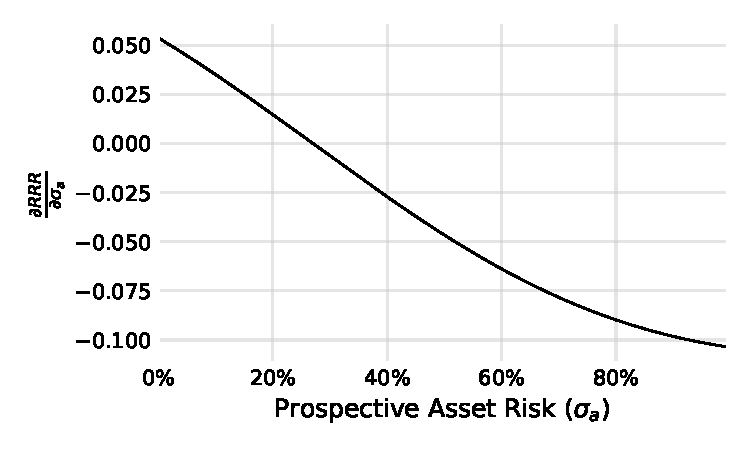
\includegraphics{paper_files/figure-latex/Partial-1} \end{center}

Focus on the portion of the curve where the partial is greater than zero
(corresponding to prospective asset risks of less than about 30\%).
Within this positive region, we know that a small increase in the
prospective asset risk, translates into a positive change in the
resulting portfolio's \(RRR\). A very cool result.

\hypertarget{disclaimer}{%
\subsection{Disclaimer}\label{disclaimer}}

\emph{This is not a solicitation to buy or sell commodity futures or
options on commodity futures and should not be construed as such.
Futures and options trading involves substantial risk and is not for
everyone. Such investments may not be appropriate for the recipient. The
valuation of futures and options may fluctuate, and, as a result,
clients may lose more than their original investment. Nothing contained
in this message may be construed as an express or an implied promise,
guarantee or implication by, of, or from Bridge Alternatives Inc that
you will profit or that losses can or will be limited in any manner
whatsoever. Past performance is not necessarily indicative of future
results. Although care has been taken to assure the accuracy,
completeness and reliability of the information contained herein, Bridge
Alternatives Inc makes no warranty, express or implied, or assumes any
legal liability or responsibility for the accuracy, completeness,
reliability or usefulness of any information, product, service or
process disclosed.}


\end{document}
